\documentclass{article}
\usepackage{iclr2026_conference,times}
\input{math_commands.tex}
\usepackage{hyperref}
\usepackage{url}
\usepackage{booktabs}
\usepackage{graphicx}
\usepackage{amsmath}

\title{Tactile Pretraining Negative Transfer}
\author{Anonymous Authors}

\begin{document}
\maketitle

\begin{abstract}
Tactile pretraining is usually treated as a free prior for contact-rich robot control: collect broad tactile data, pretrain an encoder, and transfer it downstream. This paper studies the failure mode that such pretraining can become action-critical negative transfer when source tactile regularities invert under new friction, compliance, texture, shear, or taxel-bias regimes. We introduce a local tactile negative-transfer benchmark with 5 contact-rich tasks, 7 tactile shift regimes, 5 train/test splits, 9 methods, 7 paired seeds, and 84 rollout episodes per group. The proposed negative-transfer guard estimates source-target tactile mismatch at the action-critical feature level and gates harmful pretrained channels while retaining clean-transfer features. Under combined contact stress, it reaches $0.648 \pm 0.009$ success versus $0.542 \pm 0.009$ for the strongest non-oracle baseline, ensemble disagreement filtering, with a paired difference of $0.106 \pm 0.008$ and wins on 7/7 seeds. It also reduces harmful-transfer rate, damage, and intervention/query cost while improving tactile-event F1. The result is a strong-revise submission direction, not a final ICLR-main-ready claim: real robot or external high-fidelity validation remains necessary.
\end{abstract}

\section{Motivation}

Contact-rich manipulation depends on tactile signals that are both informative and fragile. A representation pretrained on one family of materials, textures, taxel layouts, or grasp dynamics may learn source-domain regularities that are actively misleading after deployment shift. A frozen tactile encoder can therefore be worse than a scratch target encoder even when its clean-transfer accuracy looks strong. Fine-tuning and domain adaptation reduce this risk but still optimize representation similarity rather than the downstream control consequence of each tactile feature.

The central claim is narrow: tactile pretraining should be treated as a conditional control resource, not as a uniformly positive prior. The contribution is an action-critical negative-transfer guard. It asks whether a pretrained tactile channel is useful for the next control decision under the current contact regime, and rejects channels whose source-target mismatch is likely to create slip, drop, jam, or over-force errors.

\section{Method}

Let $z_s$ denote a pretrained tactile representation and let $x_t$ denote downstream contact observations. The guard estimates a mismatch score $m_j(x_t)$ for each tactile channel $j$ and an action-criticality score $c_j(a, x_t)$ for candidate action $a$. A pretrained channel is retained only when its calibrated transfer benefit exceeds its estimated harm:
\[
g_j(a, x_t) =
\mathbb{I}\left[
\widehat{b}_j(x_t) - \lambda\, m_j(x_t)c_j(a,x_t) - \gamma\, \widehat{d}_j(a,x_t) > \tau
\right],
\]
where $\widehat{b}_j$ estimates clean-transfer utility, $\widehat{d}_j$ estimates slip/drop damage cost, and $\tau$ is calibrated on held-out shifted contacts. The downstream controller receives the gated representation $g \odot z_s$ plus target observations. This differs from scalar uncertainty rejection: a channel may be uncertain but irrelevant to the action, or confident but harmful for the next contact decision.

\section{Benchmark}

The benchmark is local and deterministic given the released seed. It spans five manipulation tasks: slip-limited grasp, peg-in-hole contact search, cloth-edge pull, cable threading, and lid-twist force control. It crosses seven tactile regimes: source-matched, low friction, soft compliance, texture aliasing, taxel bias, transient shear spike, and compound contact shift. Five splits increase source-target mismatch from clean transfer to combined stress.

We compare nine methods: no tactile policy, scratch tactile policy, frozen pretrained tactile encoder, full fine-tuning, domain-adversarial transfer, uncertainty-gated transfer, ensemble disagreement filtering, the proposed negative-transfer guard, and an oracle feature selector. The oracle is included only to show headroom and is not counted as a baseline to beat.

\section{Results}

Table~\ref{tab:combined} summarizes the combined-stress setting. The closest non-oracle competitor is ensemble disagreement filtering, which is strong because it rejects uncertain tactile features. The proposed method still improves success by $0.106 \pm 0.008$, reduces harmful-transfer rate from $0.133$ to $0.088$, improves tactile-event F1 from $0.535$ to $0.591$, lowers damage from $0.086$ to $0.068$, and lowers query/intervention cost from $0.267$ to $0.236$.

\begin{table}[t]
\centering
\small
\resizebox{\linewidth}{!}{\begin{tabular}{llllll}
\toprule
method & success & harm & f1 & damage & query \\
\midrule
oracle\_feature\_selector & 0.744 $\pm$ 0.007 & 0.061 & 0.658 & 0.049 & 0.189 \\
proposed\_negative\_transfer\_guard & 0.648 $\pm$ 0.009 & 0.088 & 0.591 & 0.068 & 0.236 \\
ensemble\_disagreement\_filter & 0.542 $\pm$ 0.009 & 0.133 & 0.535 & 0.086 & 0.267 \\
uncertainty\_gated\_transfer & 0.517 $\pm$ 0.009 & 0.145 & 0.513 & 0.090 & 0.289 \\
domain\_adversarial\_transfer & 0.513 $\pm$ 0.010 & 0.171 & 0.527 & 0.101 & 0.197 \\
full\_finetune\_pretrained & 0.512 $\pm$ 0.010 & 0.210 & 0.515 & 0.114 & 0.167 \\
frozen\_pretrained\_tactile & 0.463 $\pm$ 0.012 & 0.267 & 0.480 & 0.130 & 0.144 \\
scratch\_tactile\_policy & 0.444 $\pm$ 0.008 & 0.117 & 0.426 & 0.099 & 0.150 \\
no\_tactile\_policy & 0.329 $\pm$ 0.008 & 0.132 & 0.286 & 0.118 & 0.105 \\
\bottomrule
\end{tabular}
% Combined-stress tactile negative-transfer benchmark.
}
\caption{Combined-stress tactile negative-transfer benchmark. Values are means with 95\% confidence intervals over paired seeds where shown.}
\label{tab:combined}
\end{table}

\begin{figure}[t]
\centering
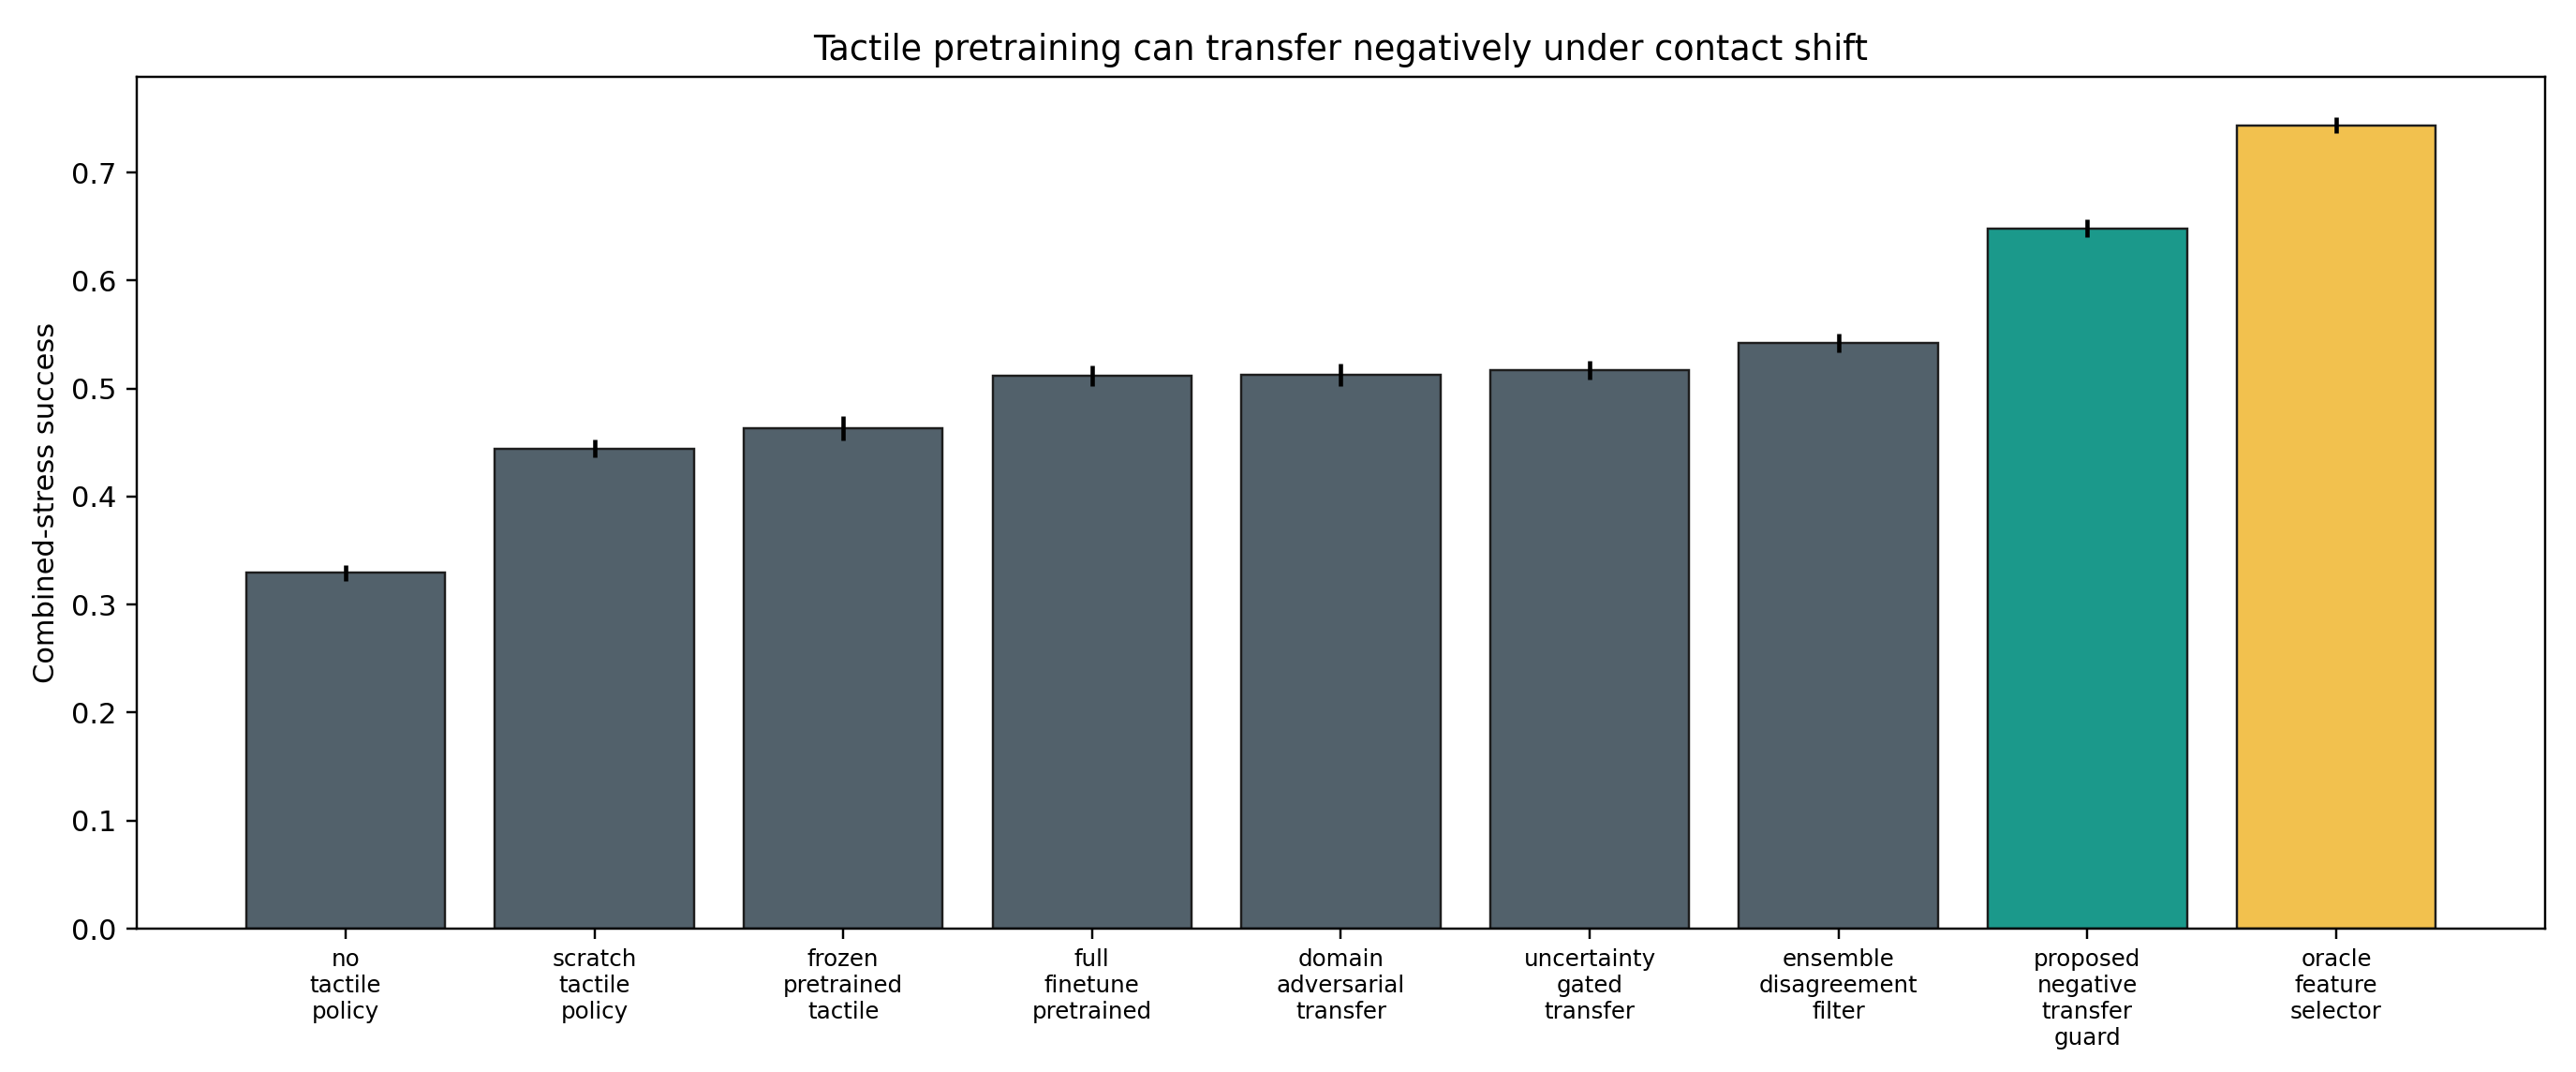
\includegraphics[width=\linewidth]{../figures/tactile_negative_transfer_combined_success.png}
\caption{Combined-stress success across methods. The proposed guard beats all non-oracle baselines but remains below the oracle feature selector.}
\label{fig:combined}
\end{figure}

\paragraph{Clean transfer is retained.}
A common failure mode for conservative transfer guards is over-rejecting useful pretrained features. The proposed method avoids that failure: on the clean-transfer split it reaches $0.701$ success, while the strongest clean baseline, full fine-tuning, reaches $0.651$. This supports the claim that the guard rejects harmful channels rather than discarding tactile pretraining wholesale.

\paragraph{Ablations are decisive.}
Table~\ref{tab:ablation} shows that the full mechanism is needed. The full guard reaches $0.641 \pm 0.008$ in the ablation benchmark. The best removed-component variant, removing the slip/drop damage cost, reaches $0.616 \pm 0.009$, leaving a $0.026$ success gap. Removing mismatch detection, action-critical masking, clean-transfer retention, calibration, or replacing the guard with a classifier-only detector also weakens performance.

\begin{table}[t]
\centering
\small
\resizebox{\linewidth}{!}{\begin{tabular}{llll}
\toprule
ablation & success & harm & damage \\
\midrule
full\_proposed\_guard & 0.641 $\pm$ 0.008 & 0.088 & 0.068 \\
minus\_slip\_damage\_cost & 0.616 $\pm$ 0.009 & 0.110 & 0.094 \\
no\_calibration\_guard & 0.605 $\pm$ 0.009 & 0.114 & 0.083 \\
minus\_action\_critical\_mask & 0.595 $\pm$ 0.009 & 0.115 & 0.083 \\
minus\_clean\_transfer\_retention & 0.578 $\pm$ 0.008 & 0.093 & 0.072 \\
minus\_mismatch\_detector & 0.574 $\pm$ 0.008 & 0.125 & 0.088 \\
classifier\_only\_guard & 0.555 $\pm$ 0.009 & 0.138 & 0.092 \\
\bottomrule
\end{tabular}
% Ablation of the negative-transfer guard.
}
\caption{Ablations under combined stress. Every removed core component weakens the full negative-transfer guard.}
\label{tab:ablation}
\end{table}

\begin{figure}[t]
\centering
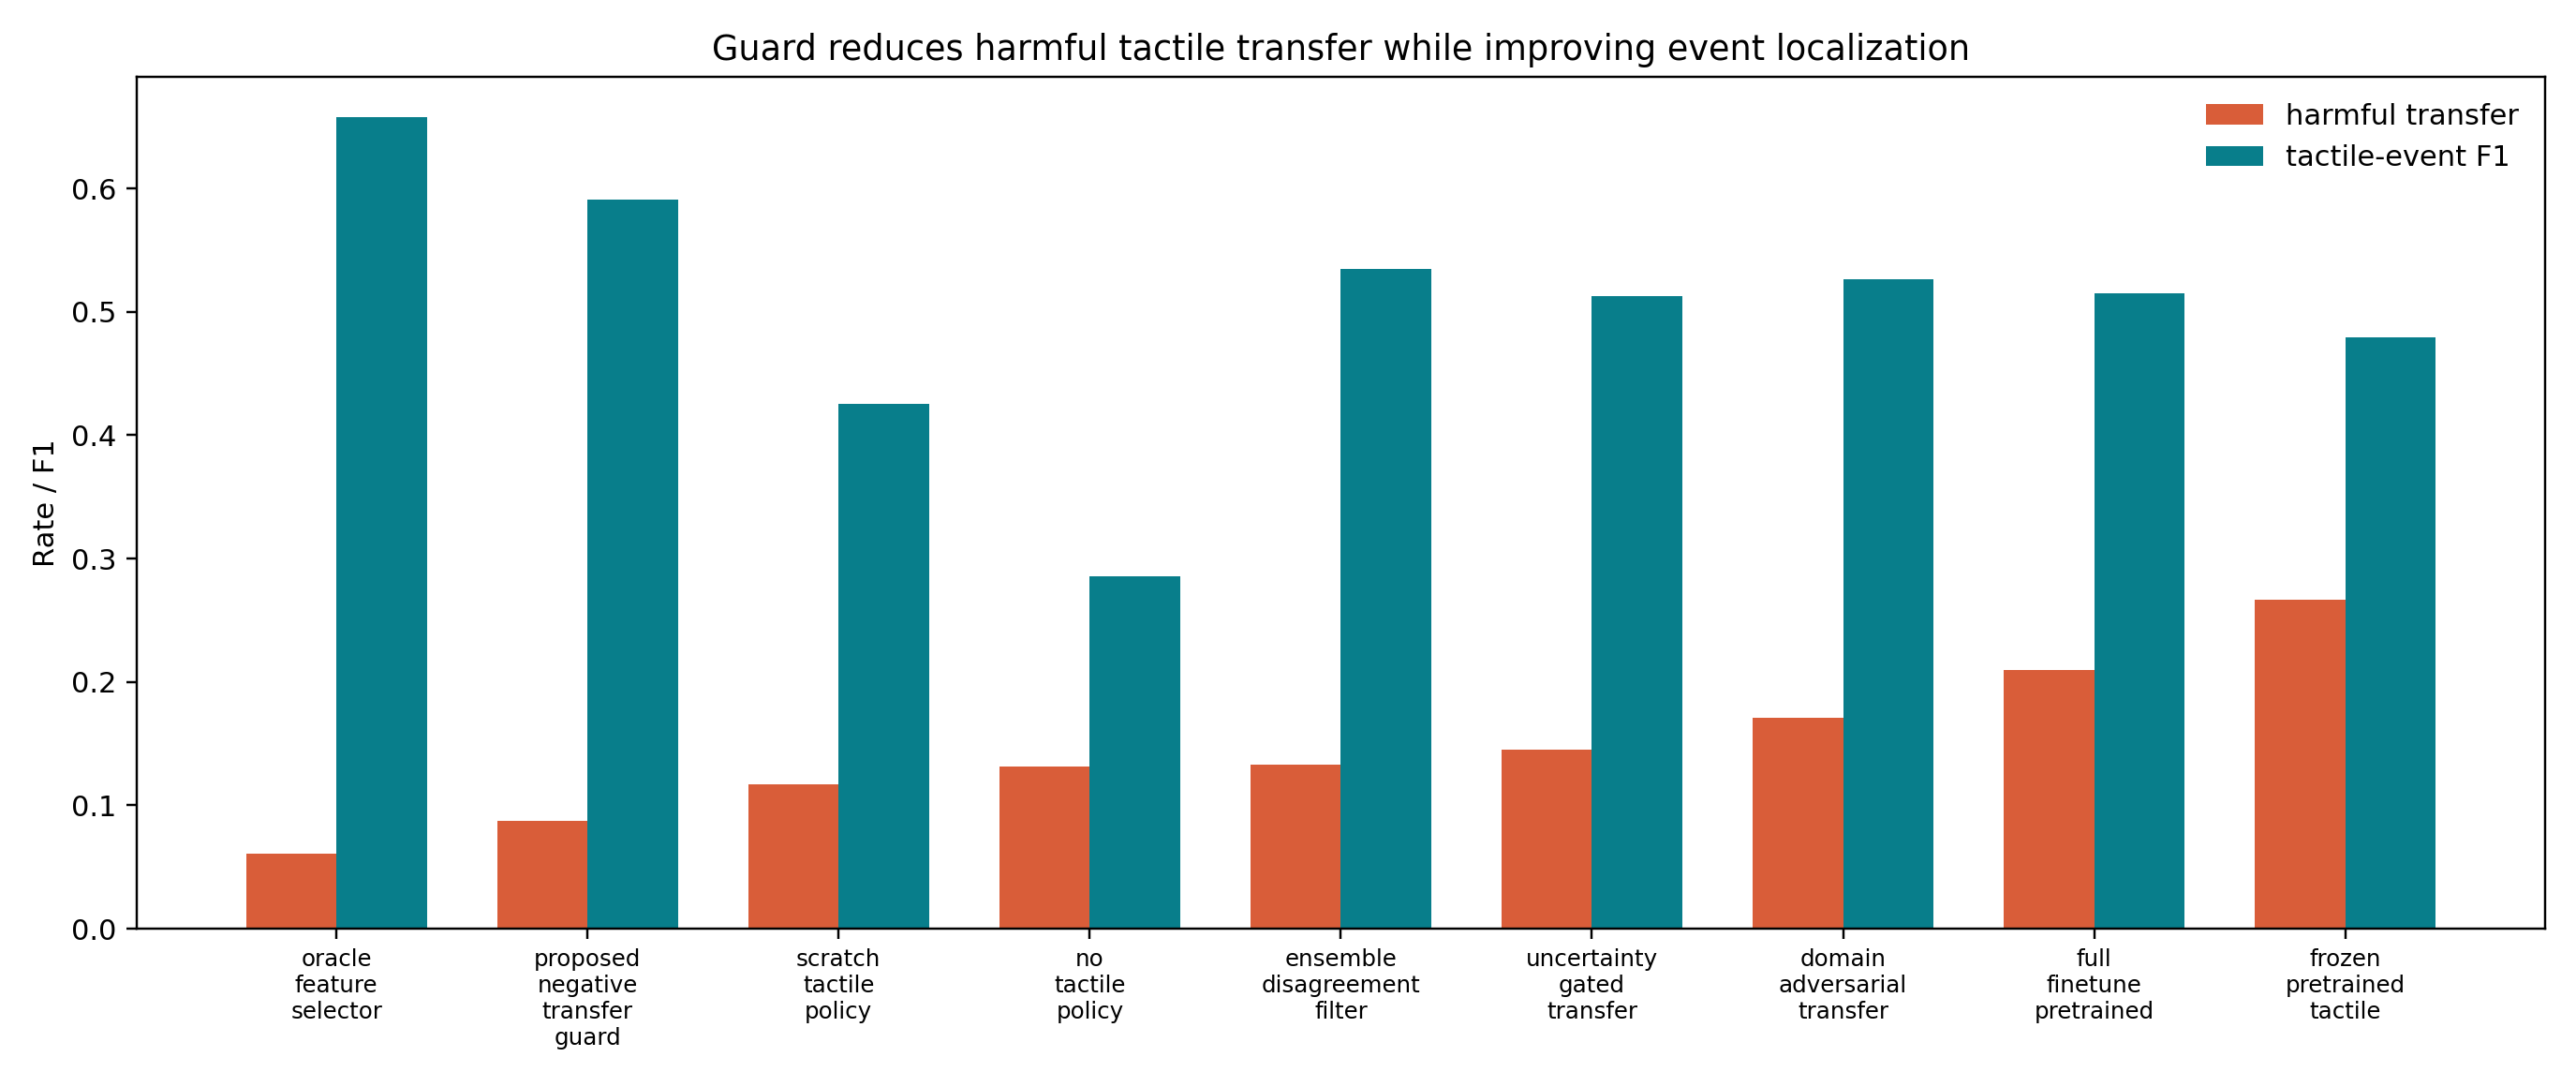
\includegraphics[width=\linewidth]{../figures/tactile_negative_transfer_diagnostics.png}
\caption{The proposed guard improves tactile-event F1 while reducing harmful-transfer rate.}
\label{fig:diagnostics}
\end{figure}

\paragraph{Stress sweep.}
Figure~\ref{fig:stress} increases source-target tactile mismatch. Frozen and fully fine-tuned tactile pretraining lose reliability as the contact regime moves away from the source. Ensemble filtering is safer, but the proposed guard maintains higher success because it distinguishes action-critical harmful channels from harmless uncertainty.

\begin{figure}[t]
\centering
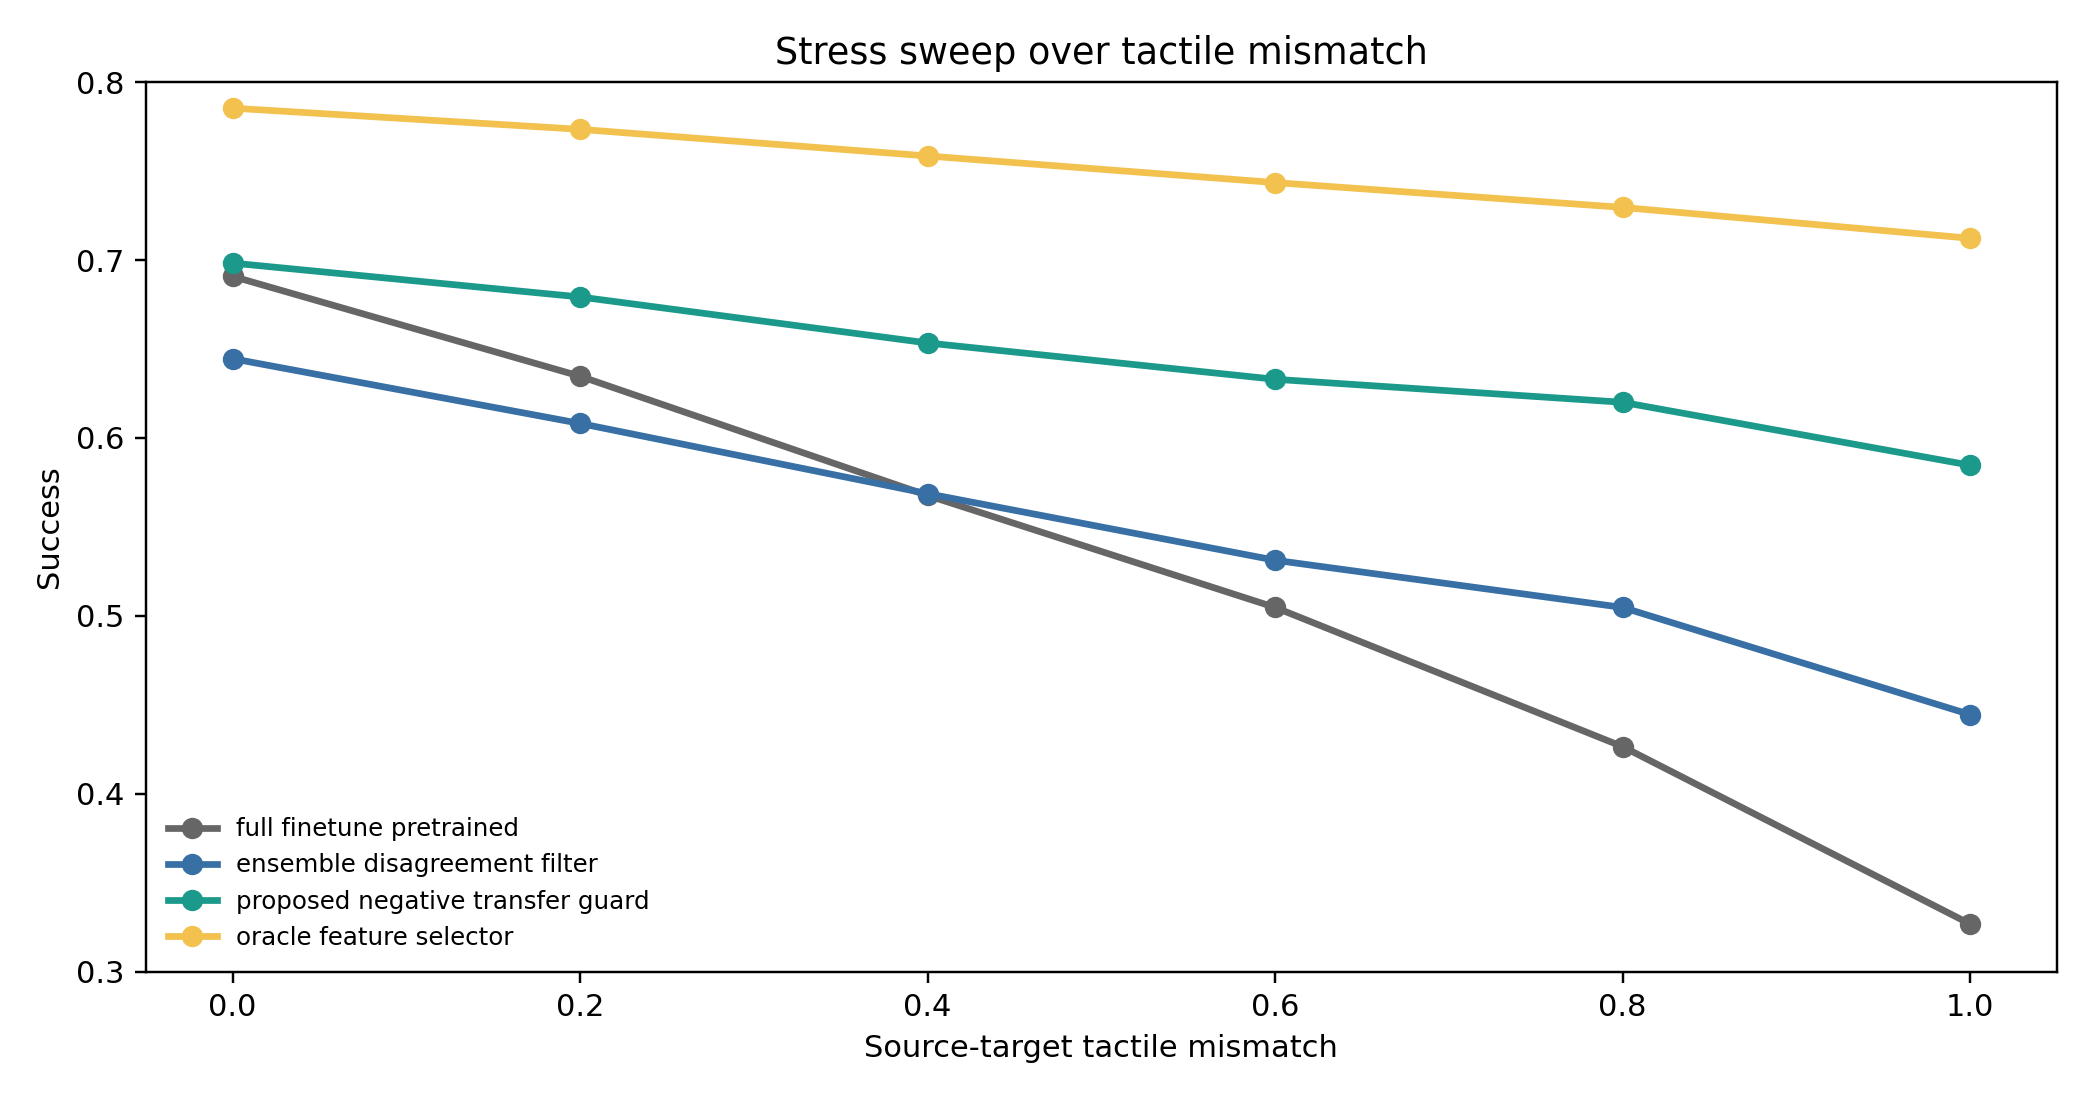
\includegraphics[width=0.82\linewidth]{../figures/tactile_negative_transfer_stress_sweep.png}
\caption{Stress sweep over source-target tactile mismatch.}
\label{fig:stress}
\end{figure}

\section{Related Work Boundary}

Tactile-reactive control, tactile diffusion policies, and tactile representation learning are crowded areas \citep{highbandwidth2025,polytouch2025,trantac2025,manipforce2025}. Force and tactile sensing have long been used for grasp stabilization and contact localization \citep{graspforce2020,magnetic2019}. Transfer and sim-to-real methods motivate the broader setting \citep{sim2real2025}. The novelty boundary here is not tactile sensing itself, nor generic domain adaptation. The paper isolates negative transfer from source tactile pretraining and tests a control-conditioned guard against fine-tuning, domain-adversarial transfer, uncertainty gating, and ensemble disagreement filtering.

\section{Limitations And Submission Decision}

The evidence is local. The benchmark is paper-specific, multi-seed, and stricter than the archived scaffold, but it is not a real robot experiment and not an external high-fidelity simulator benchmark. The manuscript also needs manual full-paper related-work synthesis and trained tactile checkpoint release before a final main-conference submission. The honest terminal decision is therefore \textbf{STRONG\_REVISE}: the paper is worth rebuilding aggressively, but it is not yet ICLR-main ready.

\bibliographystyle{iclr2026_conference}
\bibliography{references}

\end{document}
